\newpage
    \section{Messwerte}
    Die folgenden Messwerte wurden uns zur Verfügung gestellt:
    \begin{table}
\centering
\caption{Messdaten}
\label{tab:mess}
\begin{tabular}{
    S[table-format=2.0]
    S[table-format=2.1]
    S[table-format=2.2]
    S[table-format=2.1]
    S[table-format=1.1]
    S[table-format=3.0]
}
\toprule
{$t \mathbin{/} \si{\minute} $} & {$T_1 \mathbin{/} \si{\celsius} $} 
    & {$p_1 \mathbin{/} \si{\bar} $} & {$T_2  \mathbin{/} \si{\celsius} $} 
    & {$p_2 \mathbin{/} \si{\bar} $} & {$N \mathbin{/} \si{\watt} $} \\

\midrule
0  & 21.7 &   4.0   &  21.7 &   4.1  &   120 \\
1  & 23.0 &   5.0   &  21.7 &   3.2  &   120 \\
2  & 24.3 &   5.5   &  21.6 &   3.4  &   120 \\
3  & 25.3 &   6.0   &  21.5 &   3.5  &   120 \\
4  & 26.4 &   6.0   &  20.8 &   3.5  &   120 \\
5  & 27.5 &   6.0   &  20.1 &   3.4  &   120 \\
6  & 28.8 &   6.5   &  19.2 &   3.3  &   120 \\
7  & 29.7 &   6.5   &  18.5 &   3.2  &   120 \\
8  & 30.9 &   7.0   &  17.7 &   3.2  &   120 \\
9  & 31.9 &   7.0   &  16.9 &   3.0  &   120 \\
10 & 32.9 &   7.0   &  16.2 &   3.0  &   120 \\
11 & 33.9 &   7.5   &  15.5 &   2.9  &   120 \\
12 & 34.8 &   7.5   &  14.9 &   2.8  &   120 \\
13 & 35.7 &   8.0   &  14.2 &   2.8  &   120 \\
14 & 36.7 &   8.0   &  13.6 &   2.7  &   120 \\
15 & 37.6 &   8.0   &  13.0 &   2.6  &   120 \\
16 & 38.4 &   8.5   &  12.4 &   2.6  &   120 \\
17 & 39.2 &   8.5   &  11.7 &   2.6  &   120 \\
18 & 40.0 &   9.0   &  11.3 &   2.5  &   120 \\
19 & 40.7 &   9.0   &  10.9 &   2.5  &   120 \\
20 & 41.4 &   9.0   &  10.4 &   2.4  &   120 \\
21 & 42.2 &   9.0   &  9.9  &   2.4  &   120 \\
22 & 42.9 &   9.5   &  9.5  &   2.4  &   120 \\
23 & 43.6 &   9.5   &  9.1  &   2.4  &   120 \\
24 & 44.3 &   10.0  &  8.7  &   2.4  &   120 \\
25 & 44.9 &   10.0  &  8.3  &   2.4  &   120 \\
26 & 45.5 &   10.0  &  8.0  &   2.3  &   120 \\
27 & 46.1 &   10.0  &  7.7  &   2.2  &   122 \\
28 & 46.7 &   10.5  &  7.4  &   2.2  &   122 \\
29 & 47.3 &   10.5  &  7.1  &   2.2  &   122 \\
30 & 47.8 &   10.75 &  6.8  &   2.2  &   122 \\
31 & 48.4 &   11.0  &  5.6  &   2.2  &   122 \\
32 & 48.9 &   11.0  &  4.3  &   2.2  &   122 \\
33 & 49.4 &   11.0  &  3.4  &   2.2  &   122 \\
34 & 49.9 &   11.0  &  3.0  &   2.2  &   122 \\
35 & 50.3 &   11.0  &  2.9  &   2.2  &   122 \\
\bottomrule
\end{tabular}

\end{table}

    %5
    \newpage
    \section{Auswertung}
        \subsection{Aufgabenteil a)}
        \begin{figure}
               \centering
               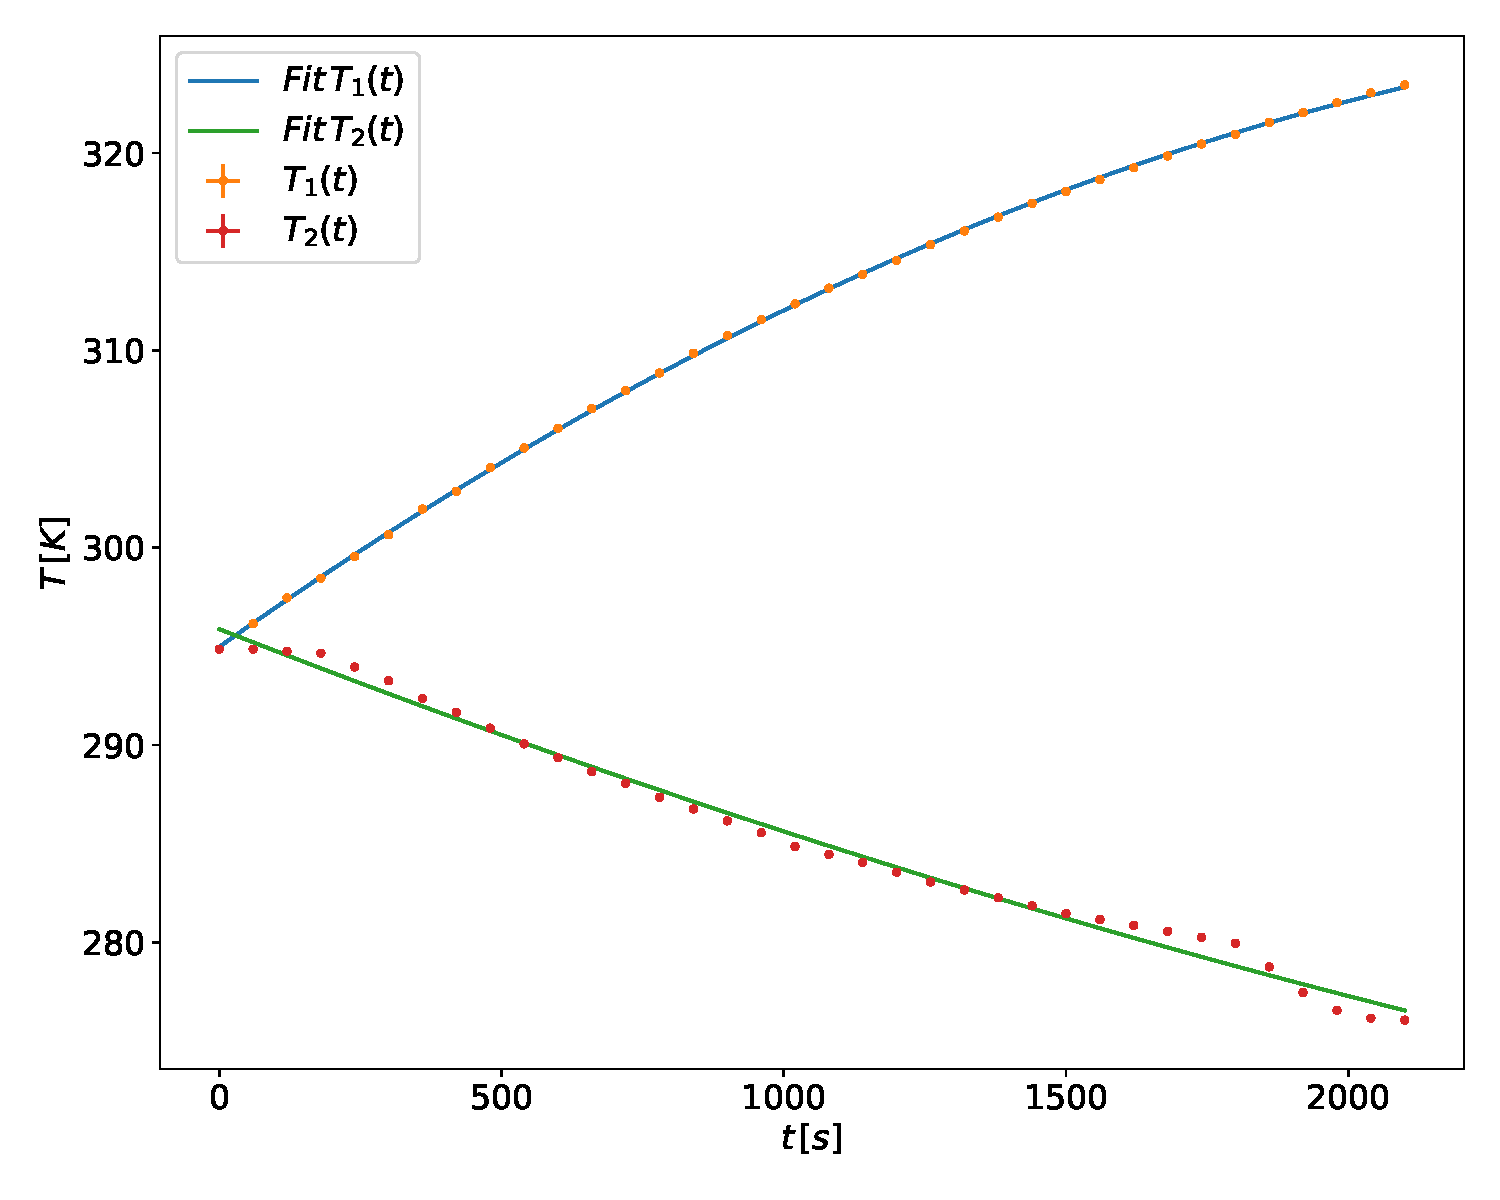
\includegraphics[width=\textwidth]{grafic.pdf}
               \caption{Auswertung mit ausgleichsgeraden}
               \label{fig:grafic}
        \end{figure}


            

        \subsection{Aufgabenteil b)}


        \subsection{Aufgabenteil c)}


        \subsection{Aufgabenteil d)}


        \subsection{Aufgabenteil e)}


        \subsection{Aufgabenteil f)}


        \subsection{Aufgabenteil g)}
        An eine ideale Wärmepumpe wird die Forderung gestellt, dass die Wärmeübertragung reversibel verlaufen muss.
Da das in der Realität nicht möglich ist, kann die vom Transportmedium aufgenommene Wärme 
und die mechanische Energie nicht jederzeit in einem umgekehrt laufenden Prozess vollständig wieder zurückgewonnen werden.
Außerdem ist davon auszugehen, dass der gesamte Aufbau durch äußere Einwirkungen beeinflusst werden und dies zu Leistungsabfällen führen kann.
Des weiteren ist zu erwähnen, dass die Isolierung den Wärmeaustausch nicht vollständig verhindert werden kann. 
Somit erfolgt auch die Kompression nicht vollständig adiabatisch.
Diese Faktoren wirken sich alle negativ auf die Güteziffer aus.